\documentclass[12pt,a4paper]{article}
\usepackage{pgf}
% \usepackage[condensed,math]{kurier}
% \usepackage[T1]{fontenc}
\usepackage{svg}
\usepackage{tikz}
\usepackage{stanli}
\usepackage{afterpage}
\usepackage{multirow}
\usepackage{subfig}
\usepackage{pgfpages}
\usepackage{svg}
\usepackage{rotating}

%\usepackage{times}


\pgfpagesdeclarelayout{boxed}
{
	\edef\pgfpageoptionborder{0pt}
}
{
	\pgfpagesphysicalpageoptions
	{%
		logical pages=1,%
	}
	\pgfpageslogicalpageoptions{1}
	{
		border code=\pgfsetlinewidth{2pt}\pgfstroke,%
		border shrink=\pgfpageoptionborder,%
		resized width=.9\pgfphysicalwidth,%
		resized height=.9\pgfphysicalheight,%
		center=\pgfpoint{.5\pgfphysicalwidth}{.5\pgfphysicalheight}%
	}%
}

\pgfpagesuselayout{boxed}


% Language setting
% Replace `english' with e.g. `spanish' to change the document language
\usepackage[english]{babel}

% Set page size and margins
% Replace `letterpaper' with `a4paper' for UK/EU standard size
\usepackage[a4paper,top=2cm,bottom=1.5cm,left=1.5cm,right=1.5cm,marginparwidth=1.75cm]{geometry}

% Useful packages
\usepackage{amsmath}
\usepackage{graphicx}
\usepackage[colorlinks=true, allcolors=blue]{hyperref}

\title{}
\author{}
\date{}

\begin{document}
	
	\newcommand{\subf}[2]{%
		{\small\begin{tabular}[t]{@{}c@{}}
				#1\\#2
		\end{tabular}}%
	}
	
	\begin{titlepage}
		\begin{center}
			
			\textbf{}
            
\includegraphics[width=1\textwidth]{utt.png}

            \vspace*{3cm}

			\vspace{1.5cm}
			
			\Huge
			\textbf{Cache with network and offline mode in PWA}
			
			\vspace{0.8cm}
			\large
			
			\vspace{0.5cm}
			\LARGE
			
			
			\vfill
			
			
			
			\vspace{0.8cm}
			
			
			
			\Large
			
			
			
			
		\end{center}
		\Large
		\begin{tabbing}
			\hspace*{1em}\= \hspace*{8em} \= \kill % set the tabbings
			\> Name:\>  \textbf{López Bautista Cristian Alexis} \\
			\> Group:\>  10-B \\
			\> Subject:\>  Progressive Web Applications  \\
			\> Professor:  \> Dr. Ray Brunet Parra Galaviz \\
			\> Date: \>  Wednesday, March 20th, 2024
		\end{tabbing}
		
	\end{titlepage}
	
    \section{Cache with Network}

    \paragraph{Cache with Network is a strategy that involves using both caching and network resources to deliver content. This strategy can be implemented in several ways, including:}

    \subsection{Cache First, Network Fallback}

    \paragraph{This strategy is also known as “Cache falling back to network”. In this strategy, the service worker first tries to fetch the resource from the cache. If the resource is in the cache, it’s returned directly to the user. If the resource is not in the cache, the service worker fetches it from the network, delivers it to the user, and adds it to the cache for future use. This strategy is useful for resources that don’t change often, like CSS or JavaScript files.}

    \begin{figure}[h!]
      \centering
      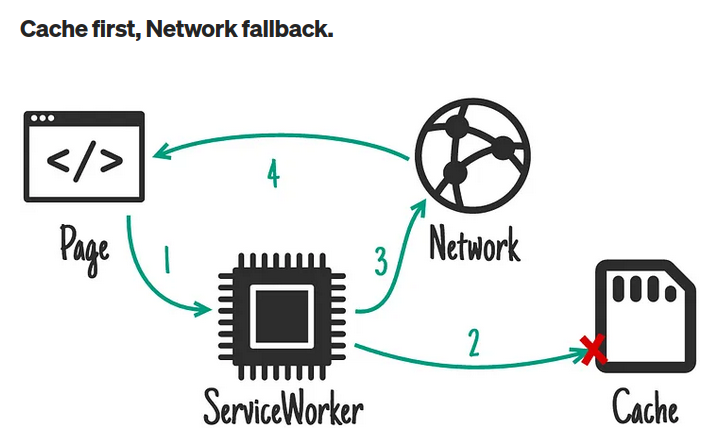
\includegraphics[width=0.5\textwidth]{cachefirst.png}
      \caption{Cache first diagram.}
    \end{figure}
    
    \subsection{Network First, Cache Fallback}

    \paragraph{This strategy is also known as “Network falling back to cache”. In this strategy, the service worker first tries to fetch the resource from the network. If the network request is successful, the response is delivered to the user and also updated in the cache. If the network request fails (for example, because the user is offline), the service worker fetches the resource from the cache and delivers it to the user. This strategy is useful for resources that change frequently or need to be up-to-date, like a news article or a social media feed.}

    \begin{figure}[h!]
      \centering
      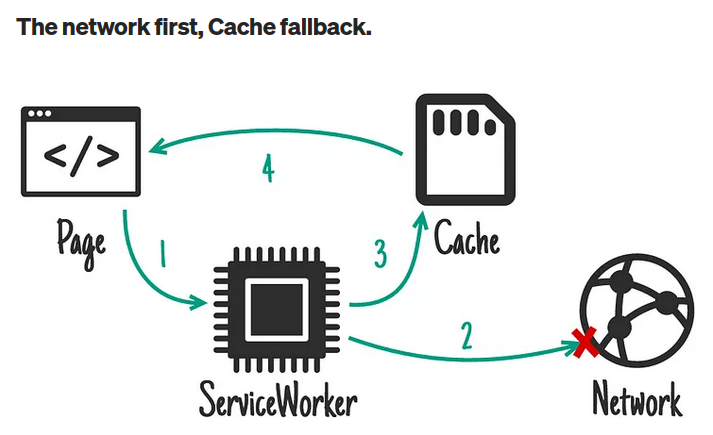
\includegraphics[width=0.5\textwidth]{networkfirst.png}
      \caption{Network first diagram.}
    \end{figure}
    
    \subsection{Stale While Revalidate}

    \paragraph{In this strategy, the service worker first delivers the resource from the cache (if available) to the user, making for a fast response. In the background, the service worker fetches the resource from the network and updates the cache. This means that the user might get stale data on the first load, but subsequent loads will have the most up-to-date resource. This strategy is useful for resources where speed is more important than freshness, like static assets or an app shell.}

    \begin{figure}[h!]
      \centering
      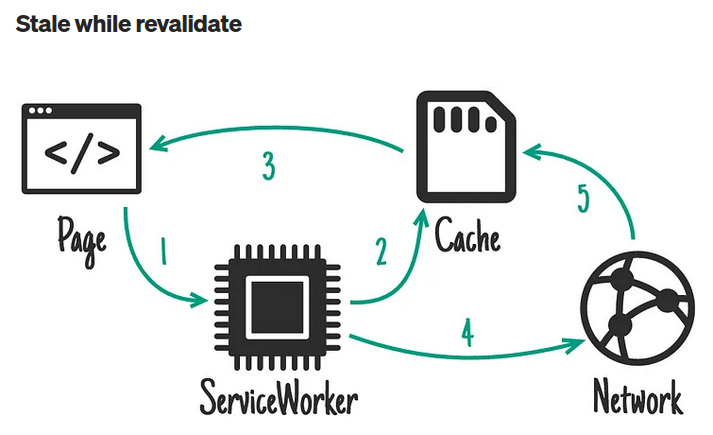
\includegraphics[width=0.5\textwidth]{stale.png}
      \caption{Network first diagram.}
    \end{figure}

    \paragraph{Each of these strategies has its own strengths and weaknesses, and the choice of strategy depends on the specific needs of your application and the nature of the resources being requested. For example, for resources that need to be up-to-date, a network-first strategy might be more appropriate, while for resources that don’t change often, a cache-first strategy could be a better choice. It’s also possible to use different strategies for different types of resources in the same application. For example, you might use a cache-first strategy for your CSS and JavaScript files, and a network-first strategy for your news articles.}

    \section{Offline mode}

    \paragraph{The offline mode in Progressive Web Applications (PWAs) is a key feature that allows the app to still function even when the user’s device is not connected to the internet. This is made possible by technologies such as Service Workers and the Cache API.}

    \subsection{Service Workers}

    \paragraph{These are scripts that your browser runs in the background, separate from a web page, opening the door to features that don’t need a web page or user interaction. They can intercept network requests and manage responses, which is crucial for handling offline scenarios.}

    \subsection{Caching}

    \paragraph{Service Workers can cache important files (like HTML, CSS, JavaScript, and images) and serve them directly from the cache when the user is offline. This means that even without an internet connection, users can still load a basic version of the app.}

    \subsection{Background Sync}

    \paragraph{This feature allows a web app to defer actions until the user has stable connectivity. This is especially useful for ensuring that whatever the user wants to send is actually sent.}

    \subsection{Offline-first Architecture}

    \paragraph{In this approach, the design of the app starts with offline functionality as a core feature. The app is built with the assumption that it might not have network connectivity, and any data that needs to be updated is done so when the connection is available.}

    \subsection{App Shell Architecture}

    \paragraph{This is a design concept where the initial load of a mobile web app provides a basic shell of an app’s UI (like the header, footer, and navigation), and the content for the app is loaded after. This can ensure that users can get meaningful pixels on the screen without the network, making the app feel instant and reliably fast.}

    \section{Conclusion}

    \paragraph{In conclusion, service workers play a pivotal role in shaping the future of web
    development by bridging the gap between web and native applications. With their
    ability to provide offline functionality, efficient caching, and background
    synchronization, service workers empower developers to create web applications that
    rival the performance and user experience of their native counterparts. By embracing
    service workers, developers can deliver fast, reliable, and engaging web experiences
    that adapt seamlessly to varying network conditions. As the web continues to evolve,
    service workers will remain a cornerstone technology, driving innovation and pushing
    the boundaries of what's possible on the modern web.}

    \clearpage

	\section{Bibliography}

    \begin{enumerate}
    
      \item Babu, L. V. (2021, 27 december). Best Caching strategies — Progressive Web App (PWA). Medium.
      
    \href{https://medium.com/animall-engineering/best-caching-strategies-progressive-web-app-pwa-c610d65b2009}{https://medium.com/animall-engineering/best-caching-strategies-progressive-web-app-pwa-c610d65b2009}

      \item Caching - Progressive web apps | MDN. (2023, 25 october). MDN Web Docs.
        
      \href{https://developer.mozilla.org/en-US/docs/Web/Progressive_web_apps/Guides/Caching}{https://developer.mozilla.org/en-US/docs/Web/Progressive_web_apps/Guides/Caching}

      \item Offline and background operation - Progressive web apps | MDN. (2023, 10 december). MDN Web Docs.
      
      \href{https://developer.mozilla.org/en-US/docs/Web/Progressive_web_apps/Guides/Offline_and_background_operation}{https://developer.mozilla.org/en-US/docs/Web/Progressive_web_apps/Guides/Offline_and_background_operation}
      
    \end{enumerate}
	
	
\end{document}